\documentclass[11pt,a4paper]{article}
\usepackage[margin=23mm,headheight=14pt]{geometry}
\usepackage{amsmath,amssymb,booktabs,tabularx,longtable,array,graphicx,xcolor}
\usepackage{tikz}
\usetikzlibrary{arrows.meta,positioning}
\usepackage{hyperref,fancyhdr,microtype}
\hypersetup{colorlinks=true,linkcolor=blue!45!black,citecolor=blue!45!black,urlcolor=blue!45!black,pdftitle={Preserving Robot Skills during Continual VLA Fine-Tuning},pdfauthor={LI HaoRan}}
\newcommand{\StudentName}{LI HaoRan}
\newcommand{\StudentID}{}
\setlength{\parindent}{0pt}
\setlength{\parskip}{5.5pt}
\setlength{\emergencystretch}{2em}
\renewcommand{\arraystretch}{1.18}
\pagestyle{fancy}
\fancyhf{}
\fancyhead[L]{\small Research Report 1}
\fancyhead[R]{\small Continual Robot Learning}
\fancyfoot[C]{\thepage}
\newcolumntype{Y}{>{\raggedright\arraybackslash}X}
\title{\vspace{-1.5em}\textbf{Preserving Robot Skills during Continual VLA Fine-Tuning}\\[0.35em]\large Forgetting Mechanisms, Mitigation Strategies, and Evaluation Boundaries}
\author{\StudentName}
\date{27 November 2026}
\begin{document}
\maketitle
\begin{abstract}
Vision--language--action (VLA) policies can adapt to new manipulation tasks, yet the same updates may degrade earlier skills. This focused survey examines ten 2026 papers on continual VLA adaptation and closely related capability-retention settings. It asks which mechanisms explain forgetting and when replay, constrained optimization, representation anchoring, and reinforcement fine-tuning provide credible protection. The main finding is conditional: strong pretraining can make simple adaptation effective, but retention depends on training objectives, memory coverage, action normalization, and evaluation distribution. In-domain success, instruction following, and robustness of old tasks are distinct outcomes. The review therefore separates reported results by protocol and identifies evidence that supports, qualifies, or limits each explanation. It concludes with a controlled evaluation design that jointly measures old-task retention, new-task acquisition, out-of-distribution robustness, and resource costs. All numerical results are attributed to the original authors; no robot-training experiment is claimed here.
\end{abstract}

\section{Research question and scope}
The practical question is whether a robot can learn a new skill without losing an earlier one. For example, after learning to place a bowl on a cabinet, it should still obey an earlier instruction to place the bowl on a stove. A failure can occur even when perception remains useful and the robot can physically execute both movements. Continual fine-tuning can alter which action a familiar scene and instruction elicit.

This report addresses the narrower technical question: \emph{which changes to data coverage, optimization, and multimodal alignment explain and mitigate skill loss during sequential VLA adaptation?} The principal outcome is retention of previously learned manipulation behavior. Retention of a VLM's general question-answering ability is a related but different problem and is not treated as evidence that old robot skills survive.

The corpus comprises ten papers first posted after January 2026 and available by 27 November 2026. Sources were identified through topic searches, related-work links, and official arXiv or conference records. Selection required explicit relevance to continual VLA learning or a controlled old-capability retention experiment. The papers are heterogeneous in review status; the presence of an arXiv identifier does not establish peer review. Liu et al.'s study has an ICML 2026 proceedings record; recent preprints are retained for their direct relevance and evaluated with appropriate caution. This is a focused critical review, rather than a claim of exhaustive systematic coverage.

Most central comparisons use the approximately 3B--7B VLA family, including OpenVLA, $\pi_0$, $\pi_{0.5}$, and GR00T variants, within the course's preferred 30B range. An exact total for LifeLong-RFT's NORA-Long was not established from the inspected paper, so this preference is not certified for every system. Model size alone does not establish feasibility: training state, image tokens, action horizons, online rollouts, and teacher networks can dominate memory or runtime. Auxiliary model costs must also be counted.

\section{Technical foundations}
\subsection{What the policy learns}
A VLA policy maps observations $o$, language instruction $\ell$, and often robot state to an action or action chunk $a$:
\begin{equation}
 a\sim\pi_\theta(a\mid o,\ell).
\end{equation}
The vision encoder extracts visual information, the multimodal backbone combines it with language, and an action component produces motor commands. Autoregressive policies predict action tokens. Regression heads predict continuous chunks directly. Flow-matching heads learn a velocity field that transforms noise into actions through an integration process. These output parameterizations change the available losses and the meaning of a response-preservation constraint.

Architecture determines the object and cost of a preservation constraint. Autoregressive policies expose action-token distributions, regression heads expose continuous chunks, and flow heads predict a velocity field along a noisy action trajectory. XIA therefore matches architecture-specific teacher and student responses under identical conditioning, including flow velocities. ConSFT instead scales the supervised flow-matching update without an additional reference network. Info-VLA freezes the visual--language encoder while updating action-side components, so unchanged encoder weights alone do not establish preserved downstream control. These distinctions locate the preservation constraint; they do not demonstrate that one output architecture inherently forgets less \cite{xia,consft,info}.

In sequential learning, task datasets $D_1,\ldots,D_K$ arrive over time. At stage $k$, the full history may be unavailable. Ordinary supervised fine-tuning minimizes the new-task loss. Experience replay (ER) adds a retained subset $B_{k-1}$ of earlier demonstrations:
\begin{equation}
\mathcal L_k=\mathbb E_{D_k}[\ell_{\rm BC}]+\lambda\mathbb E_{B_{k-1}}[\ell_{\rm BC}].
\label{eq:er}
\end{equation}
This expression describes the principle; implementations may mix examples within batches or alternate whole batches. Buffer capacity and replay frequency are separate controls. Keeping more frames does not necessarily mean drawing them more frequently.

\subsection{Why new learning can damage old behavior}
For an old-task loss and update $\Delta\theta$, a local expansion gives
\begin{equation}
\Delta L_{\rm old}\approx \nabla L_{\rm old}^{\top}\Delta\theta+
\tfrac12\Delta\theta^{\top}H_{\rm old}\Delta\theta.
\label{eq:taylor}
\end{equation}
The linear term matters away from an old-task optimum. Near such an optimum, studies often approximate curvature with a Fisher matrix and analyze $g^{\top}Fg$ for a new-task gradient $g$ \cite{hu_rl,consft}. This is a local sensitivity model, not an exact prediction of closed-loop task success. A small parameter change can still cross a grasping or contact threshold.

Low-rank adaptation (LoRA) writes $W=W_0+BA$, with rank $r$ much smaller than the original matrix dimensions. It reduces the number of trainable parameters and restricts update geometry. It does not automatically reserve disjoint parameters for every task: a single reused adapter can itself forget. Its benefit must be assessed under the actual objective, rank, training schedule, and backbone.

\subsection{Measure retention and plasticity together}
Let $R_{k,i}$ be success on task $i$ after learning through task $k$. A transparent final-checkpoint summary is
\begin{align}
 A_K&=\frac1K\sum_{i=1}^K R_{K,i},\\
 F_K&=\frac1{K-1}\sum_{i=1}^{K-1}(R_{i,i}-R_{K,i}).
\end{align}
Here $F_K$ is signed acquisition-to-final forgetting; negative values indicate improvement. It is a reporting convention for this review, not a claim that all source papers use this exact formula. Some average forgetting over every later checkpoint, while others use the final checkpoint. Signs also differ between backward transfer and negative backward transfer. Values from these definitions cannot be placed on a single leaderboard without recomputation.

Low forgetting is insufficient if acquisition was poor. A policy that never learns a task cannot lose much measured performance. A complete evaluation should therefore retain the task-by-checkpoint matrix, acquisition scores, final success, and the precise metric definition.

\section{Evidence map}
Table~\ref{tab:map} groups the corpus by the mechanism each paper investigates. The comparisons below concern reported experiments, not results produced for this report.
\begin{table}[htbp]
\centering\small
\begin{tabularx}{\textwidth}{@{}p{29mm}YY@{}}
\toprule
Study & Mechanism or intervention & Main boundary for interpretation\\
\midrule
Liu et al. \cite{liu_er} & Pretraining, ER, component swapping, skill recovery & Simulated suites; sample counts and initial ability matter\\
Hu et al. \cite{hu_rl} & Pretrained VLA + LoRA + on-policy RL & Interactive RL differs from offline imitation\\
Zhu et al. \cite{zhu_real} & Physical task streams, ER schedule, action normalization & Stepwise scores; fixed robot platforms\\
ConSFT \cite{consft} & Confidence-weighted supervised gradients & Mainly target adaptation and held-out prior skills\\
PHASER \cite{phaser} & Phase-balanced memory and interference routing & Phase sourcing; bounded but not exactly equal memory\\
XIA \cite{xia} & Old-instruction response anchoring & Additional teacher queries and temporary storage\\
OOD analysis \cite{ood} & Old-task robustness and representation probes & One model, one training seed; correlational analysis\\
RECALL \cite{recall} & Uncertainty-guided recovery-data collection & Collection quality and replay integration are coupled\\
Info-VLA \cite{info} & Information-theoretic cross-modal constraints & Estimated alignment is a surrogate for behavior\\
LifeLong-RFT \cite{lifelong} & Reinforcement fine-tuning for continual adaptation & Reward construction and offline-data coverage matter\\
\bottomrule
\end{tabularx}
\caption{Ten-study mechanism map. Each entry contributes a distinct test or intervention; the protocols do not constitute a common leaderboard.}
\label{tab:map}
\end{table}

\section{What the central comparisons establish}
\subsection{Pretraining changes replay efficiency, rather than eliminating forgetting}
Liu et al. compare pretrained VLAs with smaller policies and examine different initialization levels within the same architecture \cite{liu_er}. Their results support a useful conditional claim: strong priors can make a small replay set substantially more effective. The controlled pretraining comparison is more informative than attributing every difference to parameter count across unrelated architectures.

The study also probes whether performance loss means complete knowledge erasure. Its component-swapping and recovery experiments support partial retention of useful representations. Table 4 reports $\pi_0$ recovery-step ratios of 0.066, 0.105, 0.067, and 0.062 across four suites. Thus recovery takes approximately 6.2--10.5\% of the original steps in those tests. The 0.105 entry is a reason to avoid repeating a blanket ``under 10\%'' claim. Fast recovery still uses old-task data and training; it does not show that the deployed policy has already recovered on its own.

\subsection{The training objective changes the apparent need for anti-forgetting machinery}
Hu et al. report strong sequential adaptation with pretrained VLAs, LoRA, and on-policy reinforcement learning \cite{hu_rl}. On LIBERO-Spatial, their Table 1 reports final average success of $81.2\pm0.4$\% and NBT of $0.3\pm0.5$ percentage points. Their ablation replaces the RL objective with SFT and reports $29.9\pm2.3$\% average success with $78.7\pm1.9$ points of NBT. The ablations support an interaction among initialization, adaptation geometry, and objective in the tested setting.

These results do not establish that offline SFT should work equally well. On-policy learning samples actions from the current policy and evaluates them through interaction; imitation learning fits external demonstrations. The distributions, supervision, and costs differ. Nor does an intuitive high-dimensional null-space argument prove that trained gradients are random or harmless. The empirical Fisher and update-geometry analyses are evidence about these models, rather than a universal theorem for all large networks.

\subsection{Real-world streams expose execution-level failures}
Zhu et al. evaluate ten physical tasks spanning single-arm and bimanual manipulation \cite{zhu_real}. In their five-task homogeneous streams, Table I reports final stepwise average scores of 31.4 versus 97.2 for sequential FT and ER in the single-arm setting, and 38.3 versus 97.2 in the bimanual setting. These are task-specific progress scores on a 0--100 scale, not binary task-success rates. Their numerical magnitude should not be directly compared with LIBERO success percentages.

The action-normalization experiment is especially relevant to mechanism. Changing normalization changes the numerical coordinate system of the target actions. Replay cannot reliably align a historical action mapping if the same physical motion receives incompatible numerical targets. Freezing first-task statistics works in the tested streams when those statistics provide adequate coverage. It is not a general solution when future actions lie outside that range. The heterogeneous experiment further motivates asymmetric rehearsal for bimanual skills. These findings qualify any claim that choosing ER alone settles continual deployment.

\section{Mitigation strategies and their trade-offs}
\subsection{Improve the content and coverage of memory}
PHASER separates memory allocation within a task from replay routing across tasks \cite{phaser}. Brief events such as a grasp may receive very few frames under uniform sampling, despite being necessary for complete execution. Equal phase support addresses this bottleneck; multimodal routing prioritizes visually and linguistically similar contexts requiring different actions. In Table 1, OpenVLA-OFT on LIBERO-Long rises from 54.6\% with ER to 85.8\% with PHASER, a 31.2-percentage-point change. The comparison permits roughly $\pm10$\% memory variation, which should be stated alongside ``matched budget.'' Main evaluations use human phase annotations, while Auto-PC is separately evaluated as an automated alternative. The study therefore supports phase-aware allocation under these protocols, rather than universal autonomous deployment without preprocessing costs.

XIA addresses a different coverage gap \cite{xia}. Reweighting a fixed replay set cannot explicitly constrain old instructions on observations that never occur with those instructions in that set. XIA pairs current observations with earlier instructions and matches the previous policy's responses:
\begin{equation}
\mathcal L_{\rm XIA}=\mathcal L_{\rm ER}+\alpha\mathbb E\!\left[d\left(r_\theta(q,\ell^-),\operatorname{sg}[r_{\theta^-}(q,\ell^-)]\right)\right].
\end{equation}
Here $q$ is the response query: an observation for direct action prediction, or the observation, noisy action chunk and flow time for a flow policy. The symbols $\ell^-$, $r$, $d$ and $\alpha$ denote an earlier instruction, policy response, response discrepancy and constraint weight; $\theta^-$ is the frozen previous policy and $\operatorname{sg}$ stops teacher gradients. The target comes from the teacher; it is not the new-task expert action relabeled as an old skill. XIA reports OpenVLA-OFT average final success across three LIBERO suites of 72.5\% with ER versus 92.6\% with anchoring. The method uses the same retained expert-frame budget but adds teacher computation and temporary anchor data. A teacher response need not be correct, and an old instruction may be infeasible in a new observation. Response preservation therefore has a useful but conditional role.

\subsection{Constrain the update without storing old demonstrations}
ConSFT weights the per-sample supervised loss using a detached exponential factor \cite{consft}:
\begin{equation}
\mathcal J=\operatorname{sg}\!\left[e^{-\mathcal L/\tau}\right]\mathcal L,
\qquad g_{\rm ConSFT}=e^{-\mathcal L/\tau}g_{\rm SFT}.
\end{equation}
This is the basic detached weighting used to explain the mechanism. The implementation also includes a weight floor, loss-scale calibration, and a temperature schedule to avoid permanently suppressing unfamiliar examples. High-loss samples contribute smaller updates under the basic rule. For a fixed local curvature matrix, the associated quadratic sensitivity scales by the square of the applied weight. This algebra does not prove bounded long-horizon behavior or guarantee that an unfamiliar but necessary skill will be learned. The paper itself notes slower acquisition of unfamiliar control primitives and no formal bound on multi-step flow trajectories.

In Table 2, $\pi_0$ prior-suite average success improves from 0.09 under SFT to 0.34 under ConSFT while target success remains 0.90. This is a 25-percentage-point retention advantage in that comparison, with substantial forgetting still remaining relative to the 0.49 base score. The experiment predominantly measures old-capability preservation during narrow target adaptation; it does not establish indefinite ten-task retention under the same protocol as replay studies.

\subsection{Alignment, active collection, and reinforcement fine-tuning}
Info-VLA combines replay with teacher-guided representation alignment and an information-theoretic consistency objective \cite{info}. The authors freeze the visual--language encoder while updating the action-side components, including fusion blocks. Table 1 reports final LIBERO-Long success of 66.6\% for ER and 73.6\% for the combined approach. Yet Table 3 reports NBT of $-4.3$ for ER and $-1.0$ for the combined method, with lower marked better. Improved final success therefore does not mean that every retention metric improves. The mutual-information estimator and representation gradient path also warrant code-level verification before interpreting the objective as a proven information-preservation guarantee.

RECALL collects recovery demonstrations from states flagged by an uncertainty-based help predictor \cite{recall}. Its online collection begins at the first flagged state; its offline alternative collects from multiple flagged simulator states. With broad replay, reported overall success is 72.4\% for the Strong INSIGHT online variant versus 60.2\% for a matched passive collector. Strong INSIGHT denotes the help predictor's training-label setting, not a claim that it is always the superior predictor. Online versus offline results of 72.4\% and 68.4\% have reported $p=0.1659$, so numerical superiority is not statistically established. Recovery-only and replay comparisons also differ in action-normalization conventions in the main setup. Their full gap cannot be attributed solely to replay. This study tests a recovery-update cycle on LIBERO-10, a narrower claim than indefinite sequential skill accumulation.

LifeLong-RFT scores sampled action chunks against expert references using token agreement, decoded pose/gripper alignment, and output-format validity \cite{lifelong}. Clipped, group-relative updates and reference-policy regularization provide an alternative to directly fitting all expert outputs. The rewards require no online environment execution, but the continual protocol still retains five demonstrations per earlier task. It is consequently distinct from both replay-free adaptation and environment-interactive RL. Table IV's four-suite AUC differences average approximately 21.9 percentage points; this is neither a relative 21.9\% increase nor a final-checkpoint success comparison. Expert-reference rewards may also penalize alternative physically valid trajectories. Across these three methods, data access, trainable modules, and optimization constraints must be considered together.

\section{Why apparently conflicting findings can coexist}
\subsection{In-domain retention and robustness of the same old task}
The OOD study reevaluates an ER-trained $\pi_0$ on LIBERO-Plus perturbations \cite{ood}. Its in-domain retention remains strong while old-task OOD performance deteriorates. Importantly, it distinguishes an initial domain-shift penalty from additional degradation after later tasks. A low OOD score alone would not establish continual forgetting; the relevant comparison follows the same task across checkpoints under the same perturbation.

The paper's linear probes find that fitting a readout within the shifted domain can recover information that an in-domain readout fails to use. This is consistent with misalignment rather than total erasure. However, its one-seed, one-model study and correlational analyses cannot establish a unique causal mechanism or prevalence across all VLAs. The appropriate conclusion is that in-domain retention is insufficient evidence of robustness in this setting, motivating broader controlled tests.

\subsection{A fair comparison requires an information-and-cost budget}
Three distinctions explain much of the apparent disagreement. First, offline imitation and online RL receive different learning signals and state distributions. Second, replay studies vary between transitions and complete episodes, per-task and fixed-total memory, and different ratios of rehearsal. A fixed amount per task still grows with the number of tasks. Third, evaluations differ in pretraining overlap, task diversity, action statistics, test distributions, and success metrics.

The same method name therefore does not establish the same experiment. ER's effectiveness in one study and a newer method's advantage over ER in another should be compared through the actual replay configuration. Additional teacher queries must count as resources even when the expert-frame budget is unchanged. Matching training steps also does not necessarily match collected interactions, FLOPs, or wall-clock time.

\section{A discriminating evaluation design}
The next useful study would test whether instruction-aware and phase-aware replay preserve \emph{robust} old behavior under controlled action statistics. This is a proposed experiment, not an experiment completed here.

The proposed study would use one publicly available VLA below 30B with a fixed initialization and documented pretraining overlap. Sequential SFT, ER, phase-aware replay, ER plus instruction anchoring, and a conservative-update baseline would share a common data protocol. Online RL would form a separate experimental arm with its interaction cost recorded. Current-task demonstrations, optimizer budgets, task orders, and evaluation seeds would be held consistent where applicable. Both per-task and fixed-total memory regimes would be reported so that storage growth remains explicit.

After every task, evaluation would cover all learned tasks in-domain and under predetermined camera, lighting, object-layout, and instruction perturbations. The resulting $R_{k,i,p}$ would index checkpoint $k$, task $i$, and perturbation $p$. A goal-confusion matrix would distinguish failure to act from execution of the wrong instruction. Reported outcomes would include acquisition and final success, forgetting, uncertainty across independent training seeds, storage bytes, teacher calls, GPU memory, and training or rollout time.

Mechanism tests would ablate phase allocation while holding the total buffer constant, replace old-instruction anchors with current-instruction anchors at equal teacher-query count, compare fixed action statistics with a causally valid incremental alternative, and test whether readout repair improves closed-loop success. Representation probes and CKA alone remain descriptive. An intervention that repairs alignment while holding other factors fixed gives stronger causal evidence.

\begin{figure}[htbp]
\centering
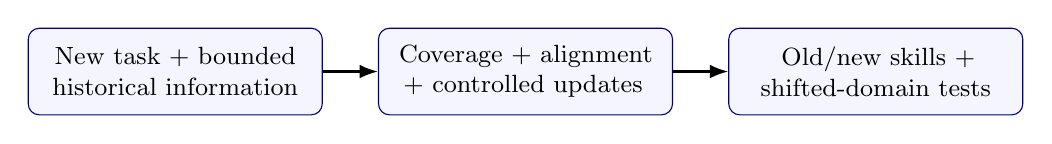
\begin{tikzpicture}[node distance=7mm, every node/.style={font=\small}, box/.style={draw=blue!50!black,fill=blue!4,rounded corners,align=center,text width=35mm,minimum height=11mm}, >=Latex]
\node[box] (data) {New task + bounded historical information};
\node[box,right=of data] (update) {Coverage + alignment + controlled updates};
\node[box,right=of update] (test) {Old/new skills + shifted-domain tests};
\draw[->,thick] (data)--(update);
\draw[->,thick] (update)--(test);
\end{tikzpicture}
\caption{Review synthesis. A retention claim is evaluated through its available information, learning intervention, and behavioral tests. This schematic contains no experimental measurements.}
\end{figure}

\section{Conclusions}
The strongest defensible conclusion is conditional retention. Pretraining and constrained adaptation can make simple continual learning surprisingly effective, yet memory coverage and execution conventions determine what is protected. Phase-aware replay targets temporal bottlenecks; instruction anchoring targets unsupervised conditional responses; conservative objectives target disruptive updates. None alone establishes general deployment reliability.

The most important unresolved issue is whether the same interventions preserve old skills when the environment shifts and when storage and interaction costs remain bounded over a long task stream. Answering it requires joint reporting of retention, acquisition, robustness, and resources. This interpretation reconciles optimistic simulation results with physical and OOD failures while preserving the distinctions in what each paper actually demonstrates.

\appendix
\section{Corpus dates, inspected versions, and publication status}
\label{app:corpus}
The inclusion date is the first public arXiv submission, not the date of a later revision. All ten studies were first posted after 31 January 2026. Dates and version numbers below were checked against the official arXiv records on 27 November 2026. The analysis cites the inspected versions. Conference association and the edition inspected are recorded separately; a later acceptance does not establish that the inspected preprint is identical to its camera-ready edition.

\begingroup
\footnotesize
\setlength{\tabcolsep}{4pt}
\begin{longtable}{@{}p{24mm}p{24mm}p{22mm}p{22mm}p{46mm}@{}}
\caption{Publication-date screening and source status.}\label{tab:corpus}\\
\toprule
Study & arXiv ID & First posted & Inspected revision & Publication evidence\\
\midrule
\endfirsthead
\toprule
Study & arXiv ID & First posted & Inspected revision & Publication evidence\\
\midrule
\endhead
\bottomrule
\endfoot
Liu et al.\ \cite{liu_er} & 2603.03818 & 4 Mar 2026 & v2, 17 Mar 2026 & ICML 2026 proceedings independently verified; analysis uses arXiv v2.\\
Hu et al.\ \cite{hu_rl} & 2603.11653 & 12 Mar 2026 & v3, 11 Jul 2026 & Official arXiv comments report acceptance at RLC 2026.\\
Zhu et al.\ \cite{zhu_real} & 2605.26820 & 26 May 2026 & v3, 8 Aug 2026 & arXiv preprint; no venue acceptance established in this review.\\
ConSFT\ \cite{consft} & 2605.08879 & 9 May 2026 & v2, 19 May 2026 & arXiv preprint; no venue acceptance established in this review.\\
PHASER\ \cite{phaser} & 2606.03598 & 2 Jun 2026 & v2, 3 Jun 2026 & arXiv preprint; no venue acceptance established in this review.\\
XIA\ \cite{xia} & 2611.31903 & 24 Nov 2026 & v1, 24 Nov 2026 & arXiv preprint, three days old at the review cutoff.\\
OOD analysis\ \cite{ood} & 2611.31511 & 23 Nov 2026 & v1, 23 Nov 2026 & Official arXiv comments report CoRL 2026 Learn@Deploy workshop presentation; this is not a main-conference proceedings claim.\\
RECALL\ \cite{recall} & 2606.23617 & 22 Jun 2026 & v1, 22 Jun 2026 & arXiv preprint; no acceptance established from the inspected record.\\
Info-VLA\ \cite{info} & 2603.13335 & 6 Mar 2026 & v1, 6 Mar 2026 & Authors' institutional publication list reports CoRL 2026; analysis uses the March preprint.\\
LifeLong-RFT\ \cite{lifelong} & 2602.10503 & 11 Feb 2026 & v2, 16 May 2026 & Authors' project cites an arXiv preprint; no venue acceptance established here.\\
\end{longtable}
\endgroup

The ICML proceedings record is available at \url{https://proceedings.mlr.press/v306/liu26bu.html}. Info-VLA's conference association is listed in the authors' institutional publication list at \url{https://milab.westlake.edu.cn/publications.html}. Other status statements refer to the corresponding official arXiv records linked in the references. ``No acceptance established'' describes this review's verification scope, not evidence that a paper was rejected or never peer reviewed.

Quality assessment therefore relies on the directness of the protocol, relevant baselines, ablations, uncertainty reporting, and reproducibility details as well as publication status. The six studies listed solely as preprints are not represented as six independently peer-reviewed publications. The two November papers provide timely, directly relevant observations but have had little time for independent scrutiny.

The preferred 30B model limit is supported for the principal familiar VLA families at the approximate level discussed in the main text. A verified exact total for NORA-Long was not obtained. Backbone parameter counts and trainable-parameter counts are not interchangeable with the total deployed policy size; auxiliary teacher, phase-segmentation, and help-prediction components also affect practical cost.

\bibliographystyle{unsrt}
\bibliography{references}
\end{document}
